\chapter{Program Development}

\section{Typical Program-generation Flow}

\begin{center}
    \textbf{Compile $\rightarrow$ Assemble $\rightarrow$ Link $\rightarrow$ Download.}
\end{center}


The generated executable file (or program image) is stored in the program
memory (normally an on-chip flash memory), to be fetched by the processor

\begin{figure}[H]
    \centering
    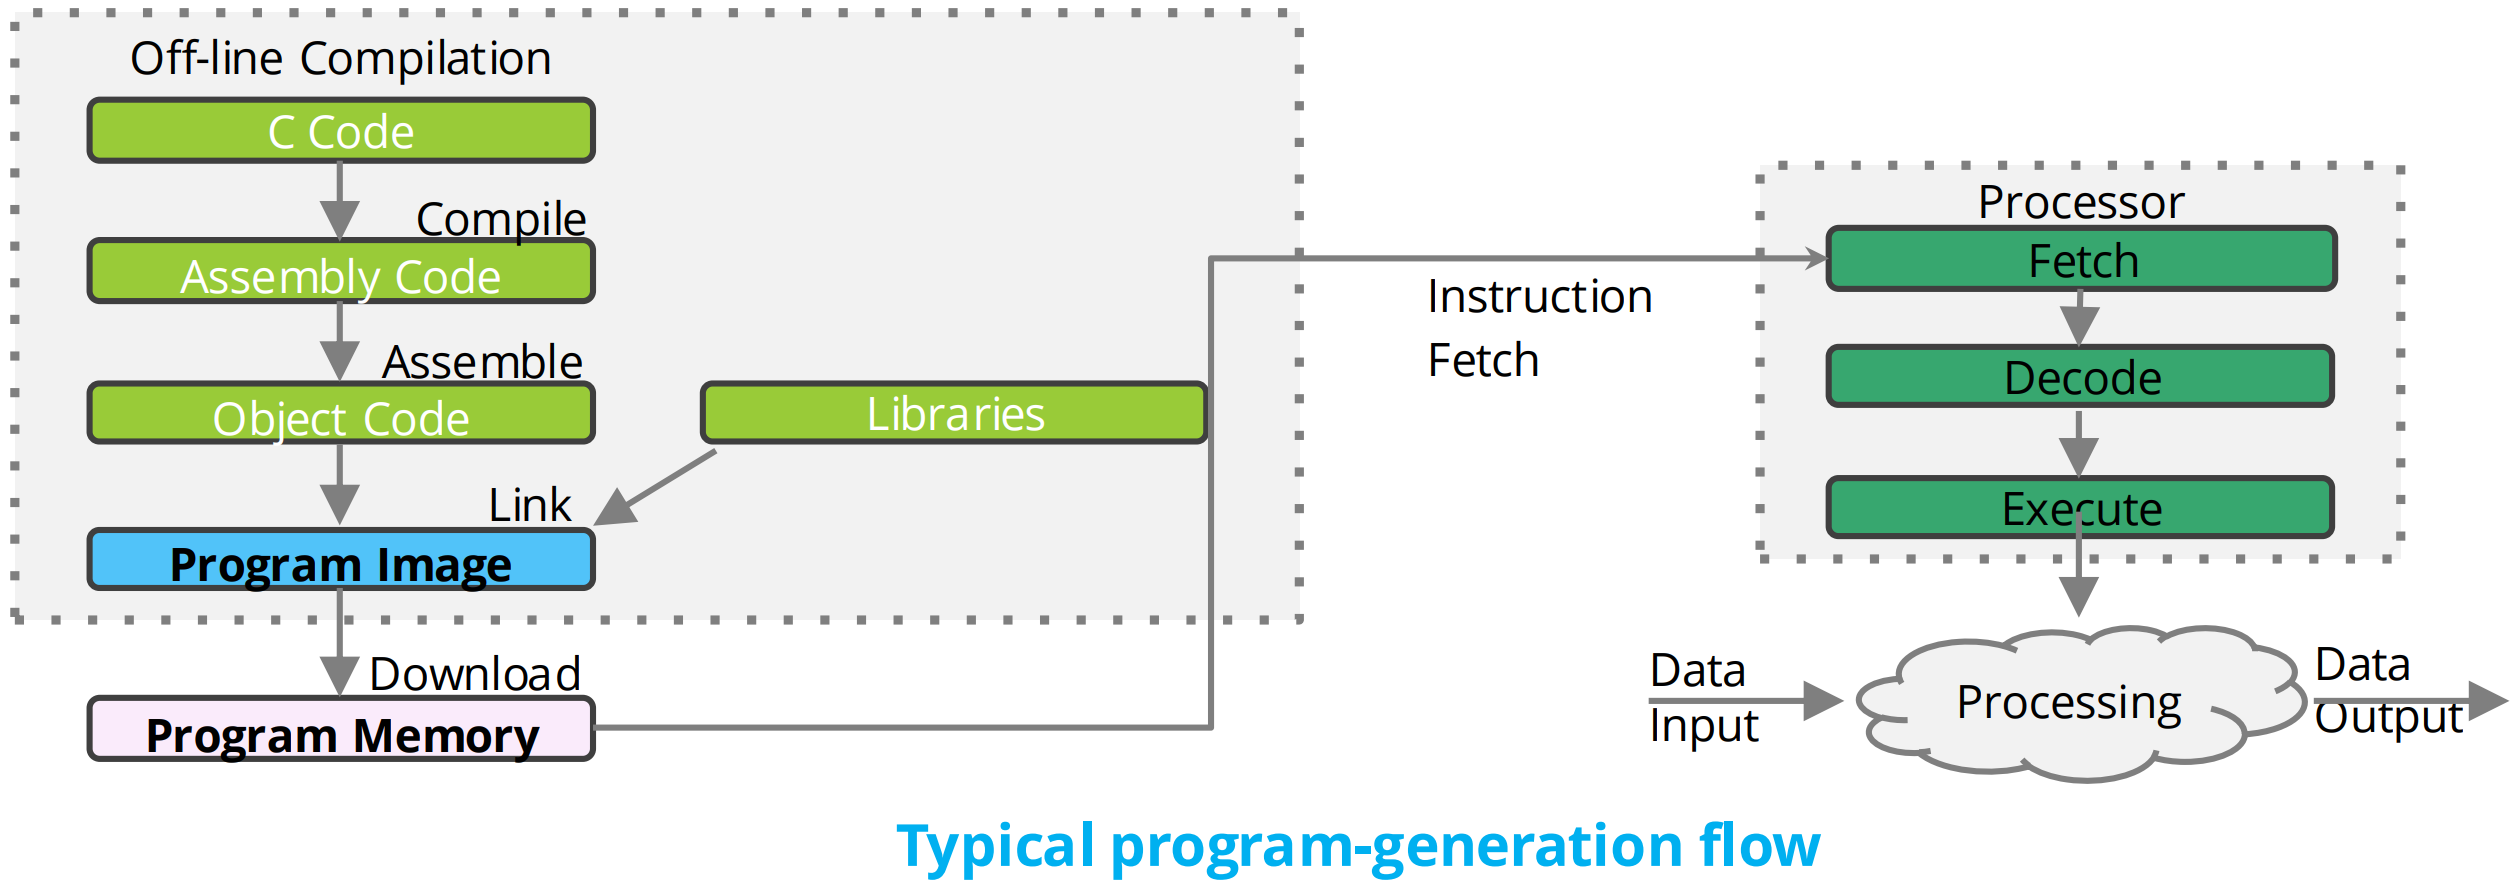
\includegraphics[width=0.85\linewidth]{img/image28.png}
\end{figure}

\section{Cortex-M4 Program Image}

A program image (or executable file) is a piece of fully integrated code that is ready to execute.


The program image includes :

 \begin{minipage}{\linewidth}
      \centering
      \begin{minipage}{0.40\linewidth}
            \begin{itemize}
                \item Program code
                \item C library code -> inserted by the linker
                \item Vector table : contains the starting addresses of interrupt vectors and the MSP (\textbf{main stack point})
                \item C startup code : used to set up data memory and initialize global variables
            \end{itemize}
      \end{minipage}
      \hspace{0.05\linewidth}
      \begin{minipage}{0.45\linewidth}
          \begin{figure}[H]
                \centering
                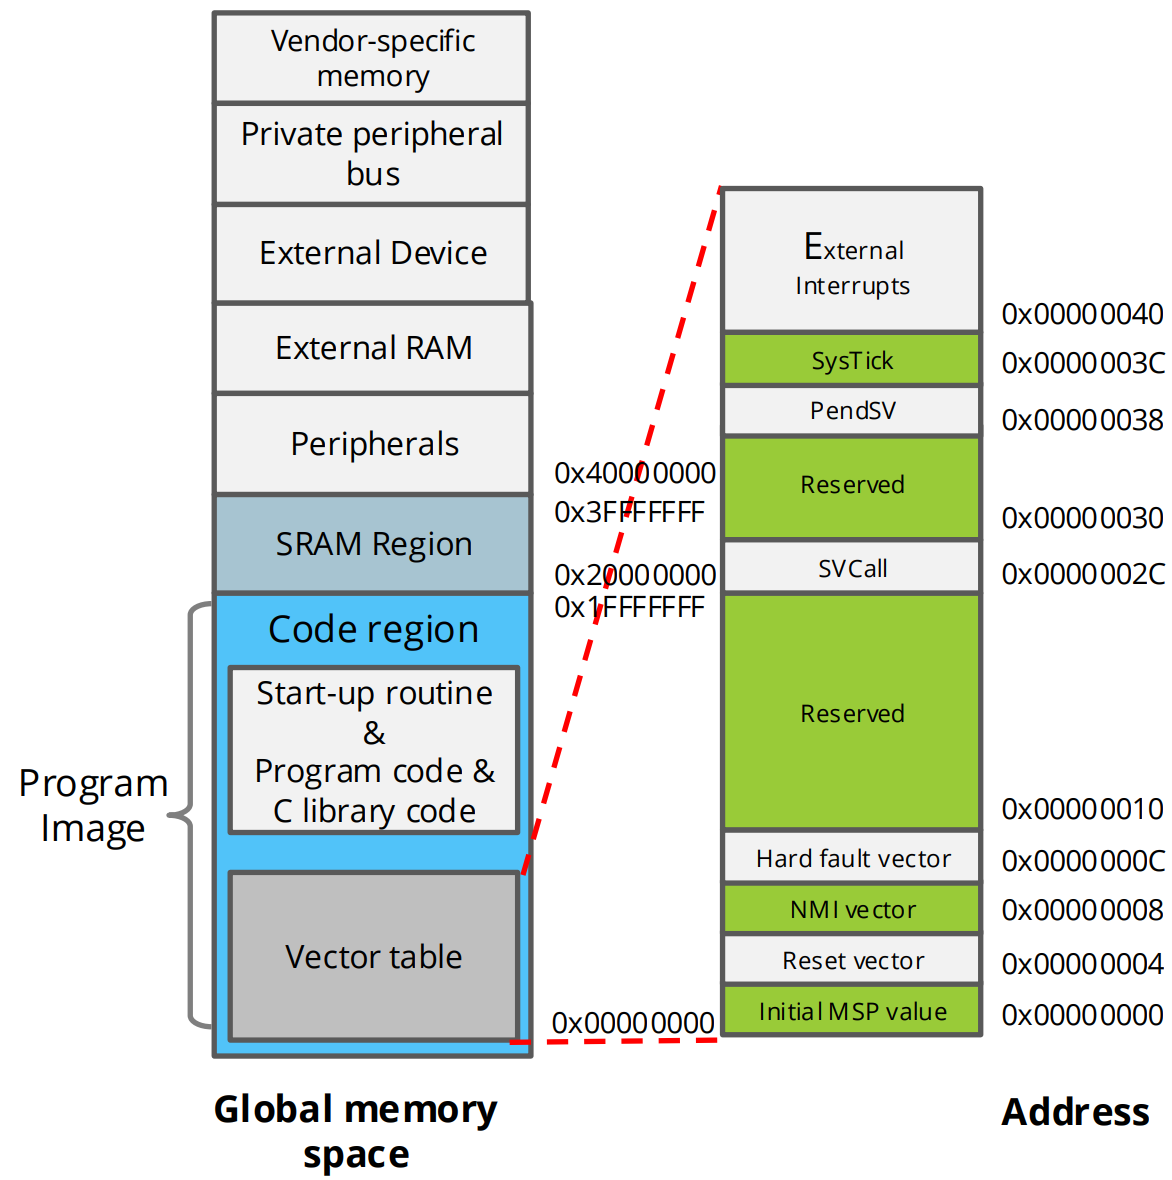
\includegraphics[width=1\linewidth]{img/image29.png}
          \end{figure}
      \end{minipage}
  \end{minipage}


\subsection{Systems Initialization}

When the system resets:

\begin{figure}[H]
    \centering
    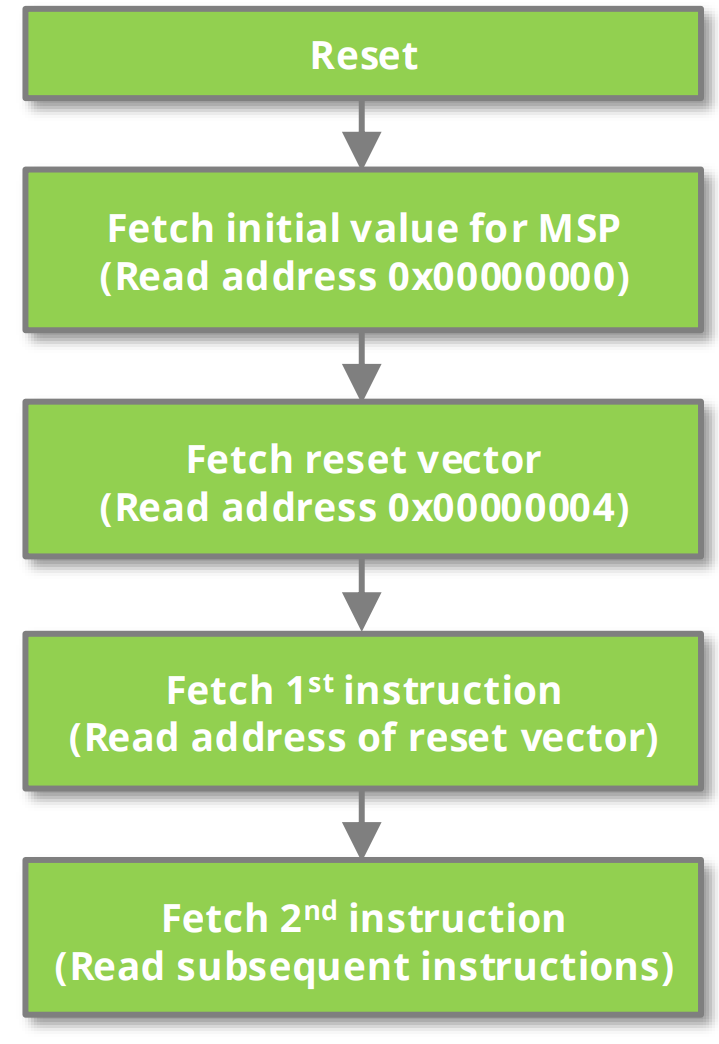
\includegraphics[width=0.23\linewidth]{img/image30.png}
\end{figure}

\section{Program Image in Global Memory}

The \textbf{program image} is stored in the code region in global memory and occupies at most 511 MB of data.

It is usually implemented on \textbf{non-volatile memory}, such as on-chip flash memory.

The executable image contains initialized data and uninitialized data. Normally separated from program data, which is allocated in the SRAM region (or data region)


\begin{figure}[H]
    \centering
    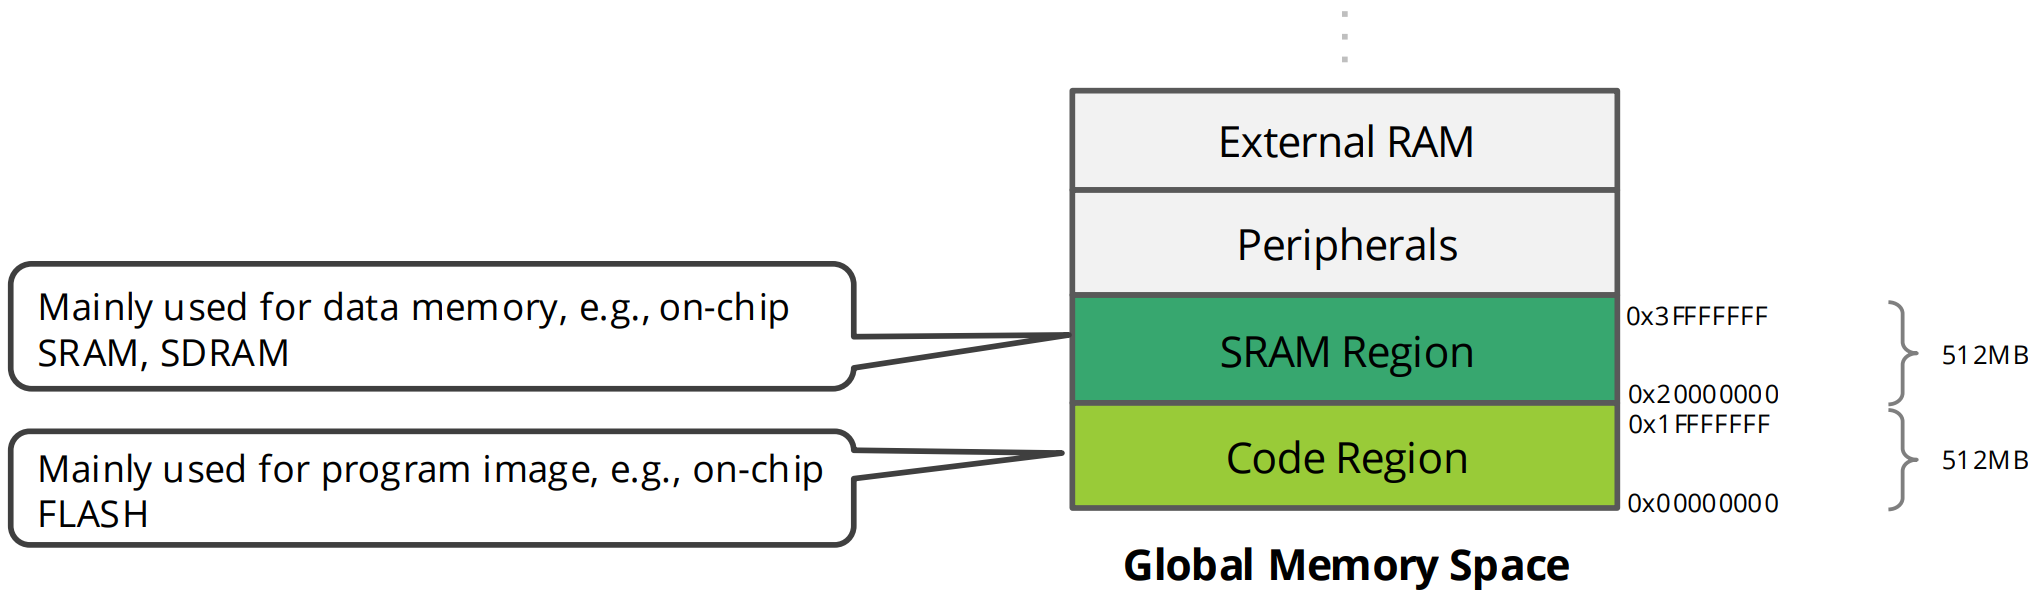
\includegraphics[width=0.8\linewidth]{img/image31.png}
\end{figure}

Normally separated from program data, which is allocated in the SRAM
region (or data region)

\section{How is Data Stored in RAM?}

Typically, the data can be divided into three
sections: \textbf{static data}, \textbf{stack}, and \textbf{heap}

 \begin{minipage}{\linewidth}
      \centering
      \begin{minipage}{0.40\linewidth}
          \begin{itemize}
            \item \textbf{Static data}: global variables and static variables
            \item \textbf{Stack}: local variables, parameter passing in function calls, registers saving during exceptions, etc.
            \item \textbf{Heap}: pieces of memory spaces that are dynamically reserved by function calls, such as ‘alloc()’ and ‘malloc ()’. (Generally not preferred in embedded systems)
        \end{itemize}
      \end{minipage}
      \hspace{0.05\linewidth}
      \begin{minipage}{0.35\linewidth}
          \begin{figure}[H]
                \centering
                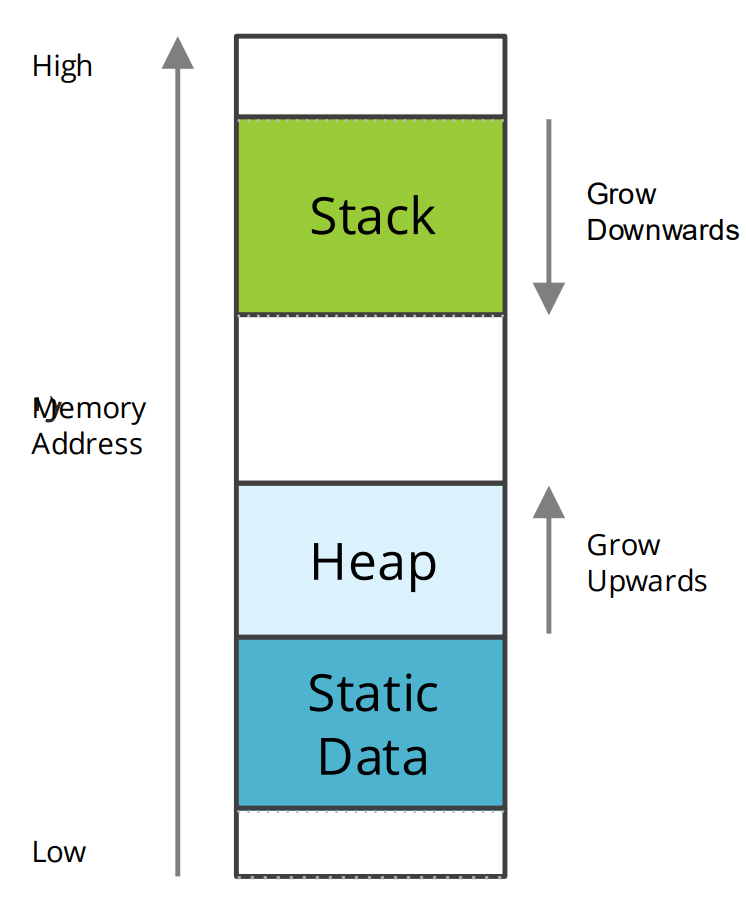
\includegraphics[width=1\linewidth]{img/image33.png}
          \end{figure}
      \end{minipage}
  \end{minipage}


\subsection{How to decide on the use of memory to store data?}

\paragraph{Information do not change: } Put it in read-only nonvolatile memory, e.g. Instructions, Constant strings, Constant
operands,
Initialization values...

\paragraph{Information change: } Put it in read/write memory, e.g. Variables, Intermediate computations,
Return address.

\begin{center}
    

\begin{lstlisting}[language=c++]
int a, b;
const char c=123; //heap
int d=31;

void main(void) {
    int e;
    char f[32];
    e = d + 7;
    a = e + 29999; //immediate value
    strcpy(f,"Hello!");
}
\end{lstlisting}
\end{center}

\begin{figure}[H]
    \centering
    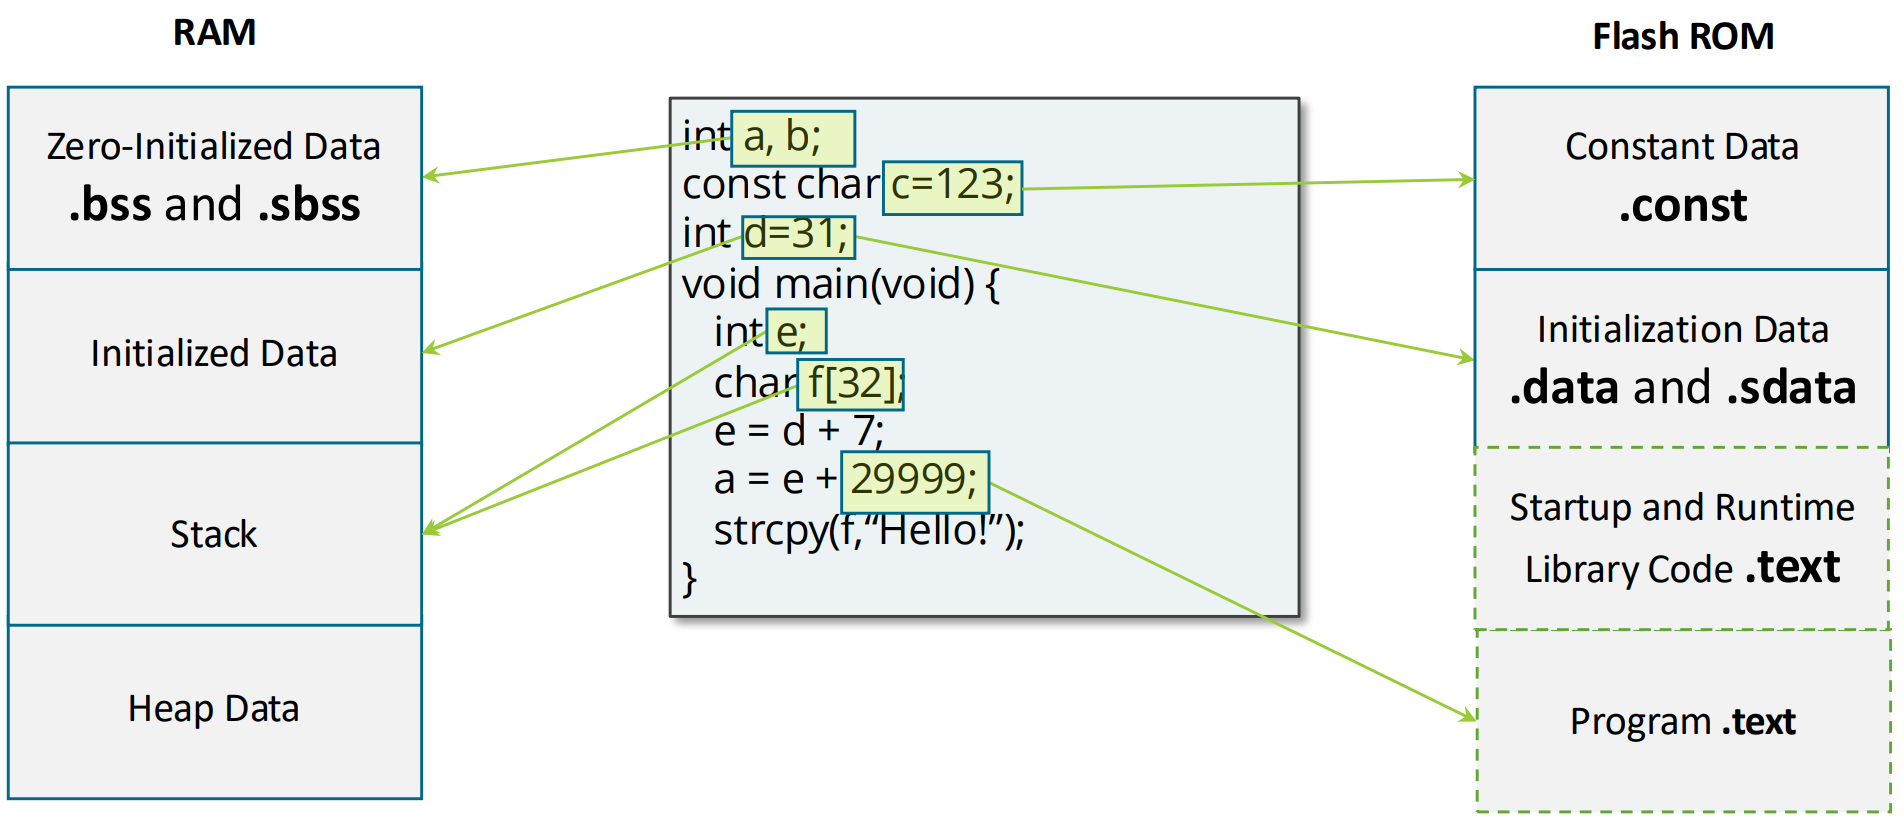
\includegraphics[width=0.85\linewidth]{img/image34.png}
\end{figure}


Executable image contains \textbf{initialized} data and \textbf{uninitialized} data sections:

\begin{itemize}
    \item .data and .sdata: contain the initial values for the global and static variables
    \item .bss and .sbss: uninitialized (or zero initialized) data sections (their content is empty)
    \item .const: constant data is part of the.const section which is read-only.
\end{itemize}


\subsection{C Run-Time Start-Up Module}

 \begin{minipage}{\linewidth}
      \centering
      \begin{minipage}{0.40\linewidth}
          After reset, MCU must: Initialize hardware... and Initialize C or C++ runtime environment: Set up heap memory, Initialize variables.
      \end{minipage}
      \hspace{0.05\linewidth}
      \begin{minipage}{0.35\linewidth}
          \begin{figure}[H]
                \centering
                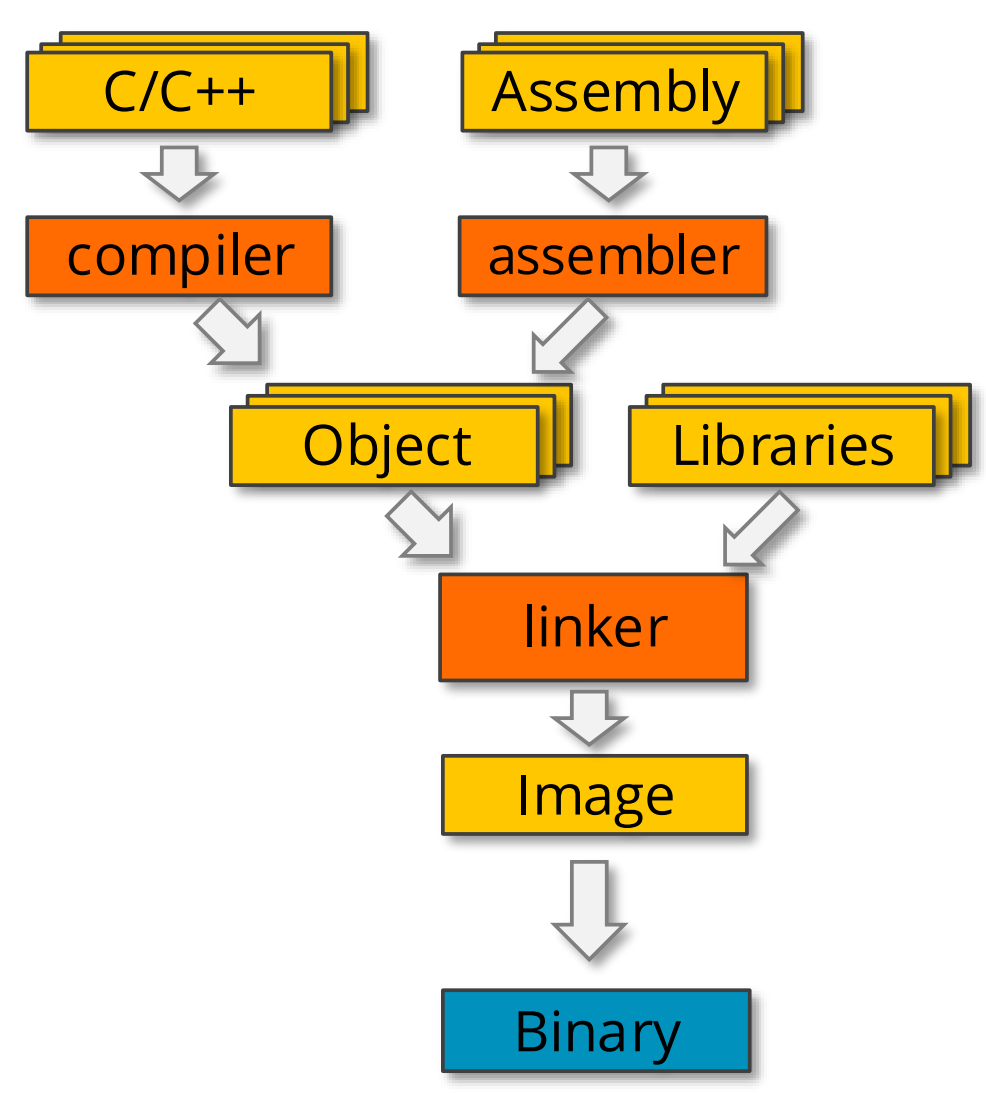
\includegraphics[width=1\linewidth]{img/image35.png}
          \end{figure}
      \end{minipage}
  \end{minipage}
  
\section{load the program mage into the target (microcontroller)}

To load a program image, we need to transfer the executable image from the host to the target (for example through an USB Cable).

There are 3 steps :

\begin{enumerate}
    \item Creating a program image in the host
    \item Loading the program image in the microcontroller using special equipment like JTAG
    \item Executing the program in the microcontroller
\end{enumerate}


\paragraph{Step one: } The linker create a single executable image for the target embedded system. 

The linker directives control how the linker combines the sections and allocates the segments into the
target system. 
Two of the more common linker directives are:

\begin{itemize}
    \item \textbf{MEMORY} : used to describe the target system's memory map, types of physical memory and address range occupied by each physical memory block
    \item[] \begin{minipage}{\linewidth}
      \centering
      \begin{minipage}{0.40\linewidth}
          \begin{figure}[H]
                \centering
                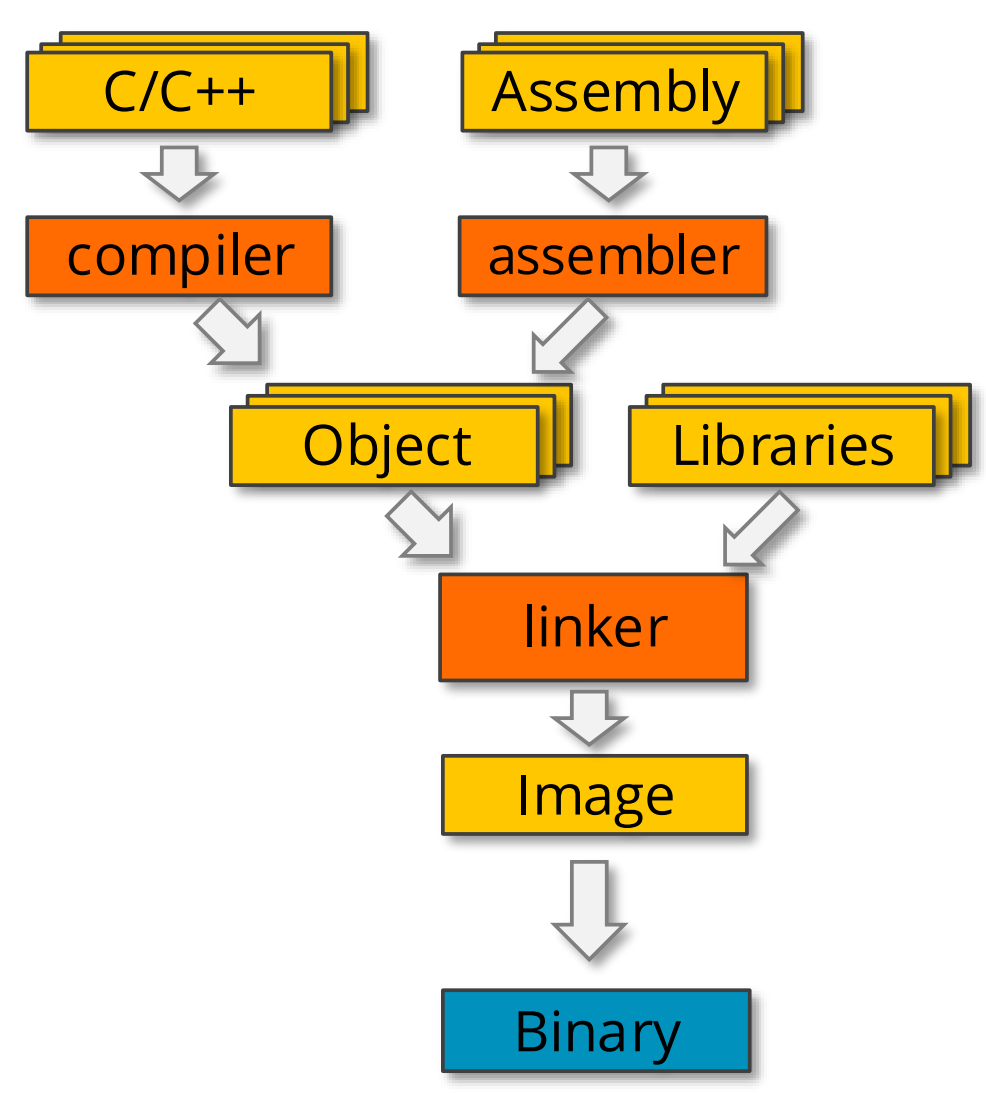
\includegraphics[width=1\linewidth]{img/image35.png}
          \end{figure}
      \end{minipage}
      \hspace{0.05\linewidth}
      \begin{minipage}{0.35\linewidth}
          \begin{figure}[H]
                \centering
                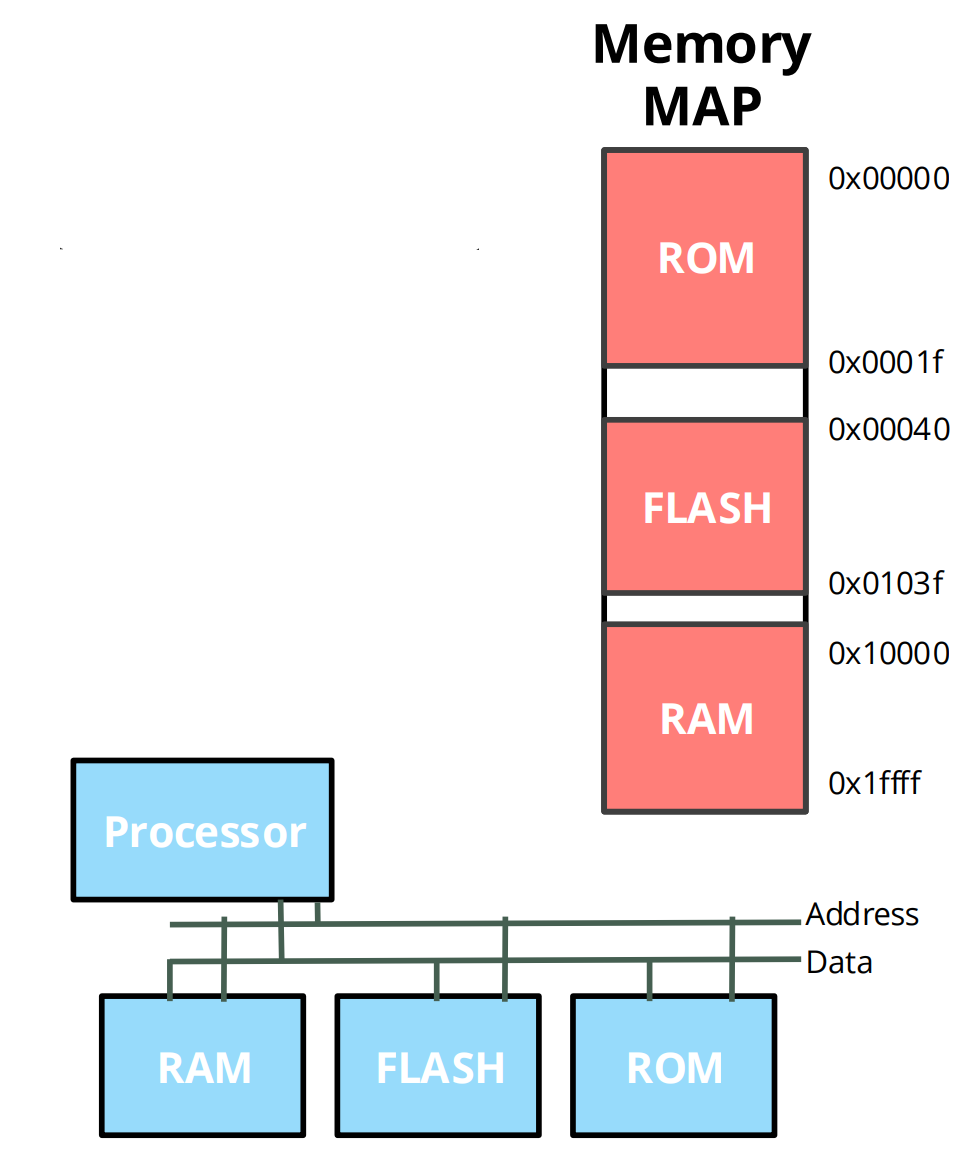
\includegraphics[width=1\linewidth]{img/image36.png}
          \end{figure}
      \end{minipage}
  \end{minipage}
  
    \item \textbf{SECTION} tells the linker:
    \begin{itemize}
    \item which input sections are to be combined into which output section
    \item which input sections are grouped together and allocated in contiguous memory
    \item where to place each section
    \end{itemize}
\end{itemize}


  \begin{figure}[H]
      \centering
      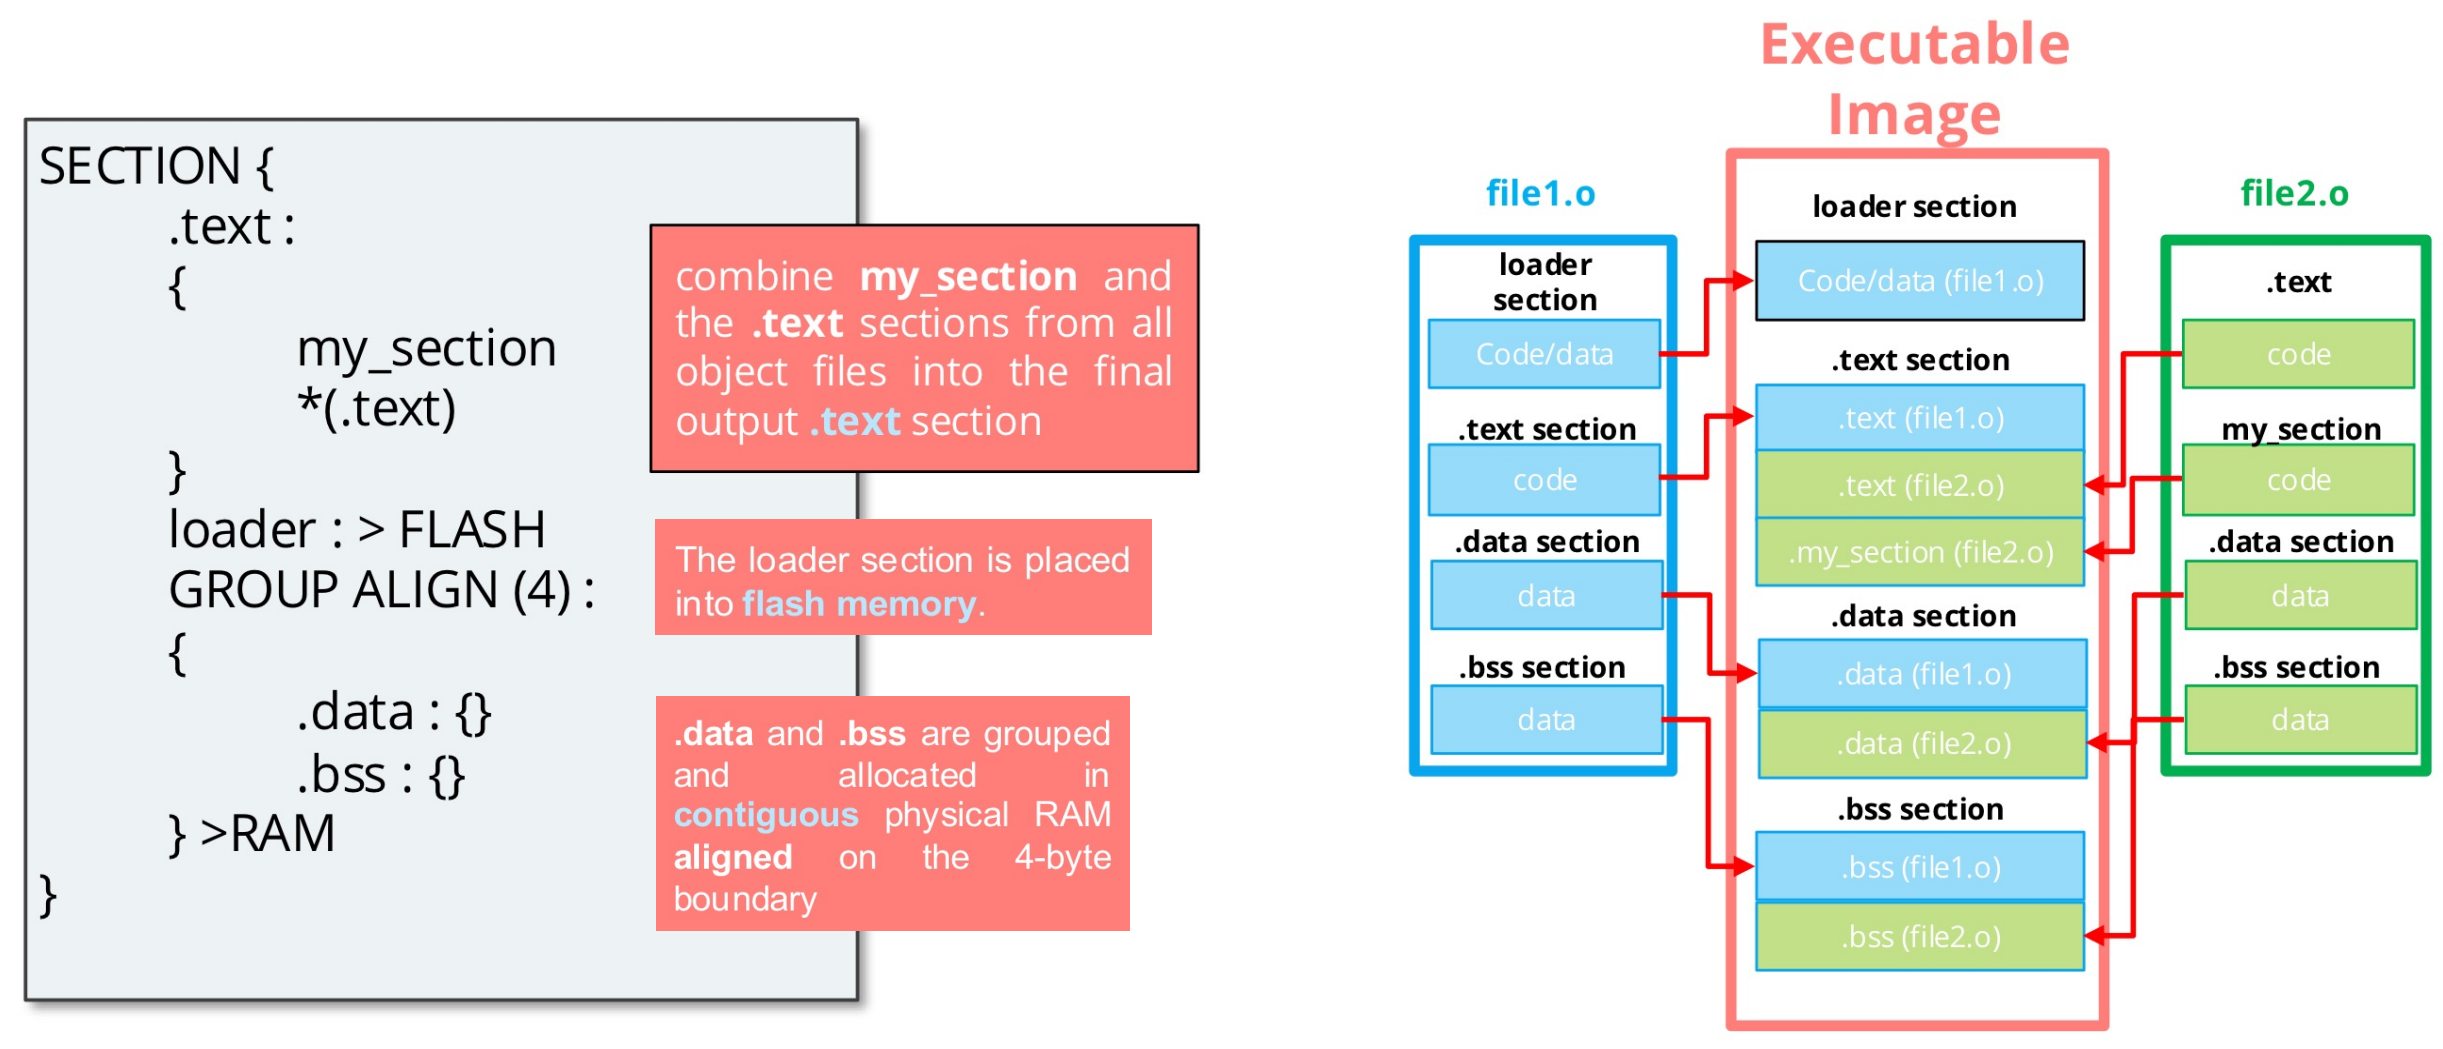
\includegraphics[width=0.9\linewidth]{img/image38.png}
  \end{figure}

  

\paragraph{Step two: }

After powered on,
the target executes code from a predefined address offset. The code in this memory location is called reset vector,
which is typically a jump instruction into the bootstrap code.

\paragraph{}
During booting, two CPU registers are concerned:

\begin{itemize}
    \item The instruction pointer register points to the next instruction (IP)
    \item The stack pointer points to the next free location in stack (SP)
\end{itemize}


\begin{figure}[H]
    \centering
    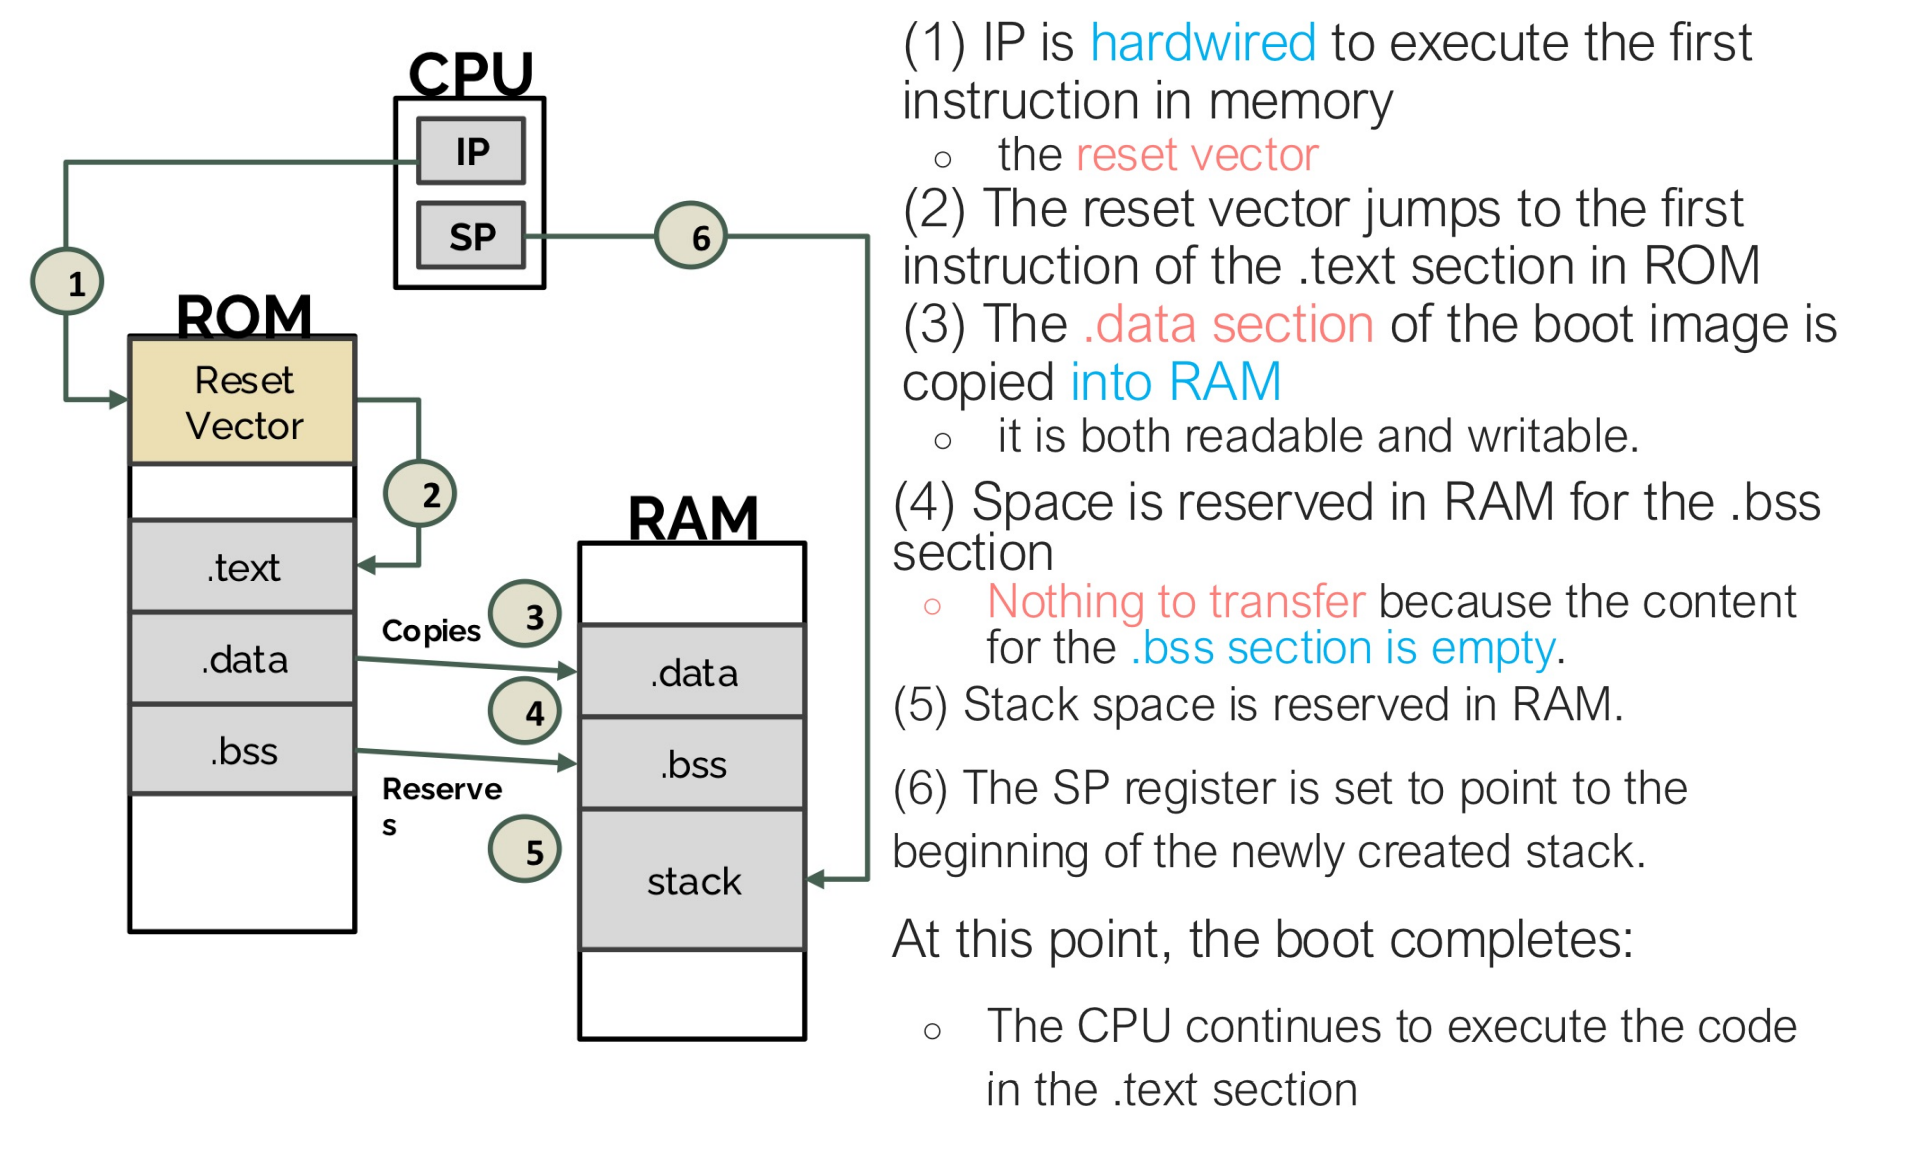
\includegraphics[width=0.9\linewidth]{img/image37.png}
\end{figure}